\documentclass{template}
\usepackage{array}
\usepackage[ngerman]{babel}
\usepackage{graphicx}
\usepackage{float}
\usepackage{csquotes}


\SetTitle{Intersektionales Wohlbefinden im Stadtraum: \\
Konzeption und Umsetzung einer App zur räumlichen Erfassung von Wohlbefinden}
\SetAuthor{\textbf{Proposal für eine Bachelorarbeit}\\
Lukas Batschelet, \href{mailto:lukas.batschelet@students.unibe.ch}{lukas.batschelet@students.unibe.ch} \\ 
Betreuung: Prof. Dr. Carolin Schurr und Dr. Moritz Gubler\\
Geographisches Institut Universität Bern}
\SetDate{\today}

\AddBibFile{references.bib}


% Hinführung, wieso ist das wichtig? Klimagerechtigkeit, warum muss man das untersuchen?
% Erwarteter Beitrag -> Bernometer wohlfülmap, erste visualisierung.
% MA Daniela Kognitive Karten von Subjektives Wohlbefinden. Eine Karte anhängen, etwa so könnte eine Karte aussehen.

% Mapping Intersectional Wellbeing in the urban
% 

\begin{document}
\maketitle




\section{Problemstellung \& Motivation}
Das Wohlbefinden im urbanen Raum hängt sowohl von räumlichen Faktoren (z.\,B.\ Infrastruktur, Grünflächen) als auch von sozialen Aspekten (z.\,B.\ Ungleichheit, Sicherheitsgefühl) ab. Studien zeigen einen engen Zusammenhang zwischen Umgebungseinflüssen und psychischer Gesundheit bzw.\ subjektivem Wohlbefinden \parencite{kan_impacts_2022, hammoud_smartphone-based_2024, bergou_mental_2022}. Zugleich verdeutlichen intersektionale Ungleichheiten – Überschneidungen von Geschlecht, Herkunft und sozioökonomischem Status – die Bedeutung sozialer Kategorien für die Wahrnehmung und Nutzung des Stadtraums \parencite{webster_centering_2021, rodo-de-zarate_developing_2014, beebeejaun_race_2022}.

Einige digitale Werkzeuge greifen diese Themen bereits auf. \emph{Urban Mind} \parencite{bakolis_urban_2018} erhebt wiederholt ortsbezogene Daten zum mentalen Wohlbefinden, verzichtet jedoch auf einen intersektionalen Ansatz. \emph{InterMaps} \parencite{rodo-de-zarate_developing_2014} integriert Intersektionalität und Raum, basiert aber auf einer einmaligen, retrospektiven Erhebung ohne laufende Geolokalisierung. Zudem sind beide Anwendungen nicht Open Source und können deshalb nicht einfach weiterentwickelt werden. Eine Anwendung, die wiederholte Erhebungen \emph{und} intersektionale Kategorien kombiniert, liegt bislang nicht vor.

Idee dieser Arbeit ist daher, eine App zu entwickeln, welche Stärken beider Tools verbindet und methodische Lücken schliesst. Durch regelmässige, ortsbezogene Befragungen, die verschiedene soziale Kategorien berücksichtigen, werden \emph{alltägliche} und intersektionale Daten zum Wohlbefinden erhoben. Gleichzeitig möchte ich meine persönliche Motivation, ein Softwareprojekt umzusetzen, einbringen und eine Anwendung schaffen, die offen genutzt und weiterentwickelt werden kann.



\section{Zielsetzung \& Fragestellungen}
Das Ziel dieser Arbeit ist die Entwicklung und Erprobung einer mobilen App, die intersektionales Wohlbefinden im Stadtraum in Echtzeit erfassen kann. Die App soll es ermöglichen, ortsbezogene Daten über subjektives Wohlbefinden unter Berücksichtigung intersektionaler Kategorien zu sammeln.

Die zentrale Forschungsfrage lautet:
% Die Frage nach der Einschränkung auf den Stadtraum stellt sich schon. Wieso genau? Evtl. auch spannend da bspw. Menschen mit Problemen in mentaler Gesundheit in Städten übervertreten sind, obwohl nachgewisen ist, dass sich der Stadtraum negativ auf die mentale Gesundheit auswirkt.
\begin{itemize}
    \item \emph{Wie kann intersektionales Wohlbefinden im Stadtraum mit einer digitalen Anwendung erfasst werden?}
\end{itemize}

Weitere Unterfragen sind:
\begin{itemize}
    \item Welche methodischen und technischen Anforderungen muss eine solche App erfüllen?
    \item Wie müssen Fragen zur Erfassung von intersektionalem Wohlbefinden formuliert sein?
    \item Wie kann intersektionales Wohlbefinden räumlich dargestellt werden?
    \item Welche Herausforderungen ergeben sich bei der Entwicklung und Testung der App?
\end{itemize}

\section{Methodisches Design}

\subsection{Fragebogenentwicklung, Datenerhebung und Pilotphase}

Ein zentraler Schritt dieser Arbeit ist die Entwicklung eines Fragebogens zur Erfassung intersektionalen Wohlbefindens im Stadtraum. Um bewährte Methoden einzubinden, wird auf bestehende Skalen zur Messung von Wohlbefinden (z.\,B.\ WHO-5, SWEMWBS, PANAS) zurückgegriffen. Ob bereits Instrumente existieren, die intersektionale Aspekte systematisch integrieren, wird im Rahmen der Literaturrecherche geklärt. Unabhängig davon werden ergänzende Items entwickelt, die verschiedene soziale Kategorien berücksichtigen und auf die subjektive Wahrnehmung bestimmter Orte und Situationen abzielen. Die Arbeit von Maria Rodó-de-Zárate \parencite*{rodo-de-zarate_intersectionality_2018, rodo-de-zarate_young_2015, rodo-de-zarate_developing_2014}
bietet hierfür relevante theoretische und methodische Anknüpfungspunkte. 

Der entwickelte Fragenkatalog wird vor der Anwendung überprüft, um Verständlichkeit, inhaltliche Passung und Anwendbarkeit sicherzustellen. Hierfür kommen etablierte Pretest-Verfahren in Frage, etwa \emph{Think-aloud}, \emph{kognitive Interviews} oder Peer-Review. Die genaue Methode wird abhängig von den verfügbaren Ressourcen gewählt. Die Ergebnisse der Überprüfung fliessen in eine optimierte Fassung des Fragebogens ein, die schliesslich in der Pilotphase getestet wird.

\subsubsection{Pilotphase}
Da diese Bachelorarbeit nur einen begrenzten zeitlichen Rahmen abdeckt, ist keine gross angelegte Studie vorgesehen. Stattdessen wird eine \textit{kurze Pilotphase} (voraussichtlich mit 5–10 Teilnehmenden) durchgeführt, um die grundlegende Funktionsfähigkeit der App und die Akzeptanz der Befragungen zu testen. Diese Pilotphase dient dazu, erste explorative Erkenntnisse über die Nutzbarkeit der Daten zu gewinnen. Folgende Ziele stehen im Vordergrund:

\begin{itemize}
    \item \textbf{Technische Validierung}: Überprüfung, ob die App stabil läuft und die Standorterfassung zuverlässig funktioniert.
    \item \textbf{Benutzerfreundlichkeit}: Einsammeln von Feedback zum Fragebogen (Verständlichkeit, Länge, Relevanz) und zur Bedienoberfläche.
    \item \textbf{Datenauswertung im Kleinen}: Erste Auswertungen der erhobenen Daten, um festzustellen, ob sich Muster erkennen lassen, wie Teilnehmende ihr Wohlbefinden in Abhängigkeit von Ort und Situation einschätzen.
    \item \textbf{Entwurf einer Visualisierung}: Aus den Daten einen Entwurf entwickeln, wie sich die Daten ansprechend und verständlich präsentieren lassen.
\end{itemize}

Eine umfassende statistische Auswertung oder repräsentative Aussagen zum intersektionalen Wohlbefinden sind in diesem Umfang \textit{nicht} realistisch. Die Erkenntnisse aus der Pilotphase können jedoch wertvolle Hinweise darauf liefern, inwieweit eine grössere Studie sinnvoll wäre. Eine solche Folgestudie könnte beispielsweise im Rahmen einer künftigen Masterarbeit oder eines anderen Forschungsprojekts durchgeführt werden.

\subsection{Technische Umsetzung}
Die App wird nach einer vorangegangenen technischen Evaluation mit \emph{React Native (Expo)} \footnote{\href{https://expo.dev/}{https://expo.dev/}} als Frontend-Technologie und \emph{Supabase}\footnote{\href{https://supabase.com/}{https://supabase.com/}} als Backend-Datenbank umgesetzt. Dies ermöglicht eine plattformübergreifende Entwicklung und eine sichere und flexible Datenverwaltung.

Mögliche Funktionen sind:
\begin{itemize}
    \item \textbf{Geolokalisierte Fragen}: Automatische Erfassung des Aufenthaltsorts
    \item \textbf{Tägliche Erinnerungen}: Drei kurze Erhebungen pro Tag
    \item \textbf{Intersektionale Kategorien}: Nutzer*innen geben einmalig demografische Informationen an
\end{itemize}

\subsubsection{Datenschutz}
Da die App sensible Daten zum Wohlbefinden und zum Standort erfasst, stehen datenschutzrechtliche Überlegungen an oberster Stelle. Folgende Prinzipien sollen sicherstellen, dass die Datenerhebung möglichst risikoarm erfolgt:

\begin{itemize}
    \item \textbf{Pseudonymisierung}: Die Teilnehmenden werden nur über eine zufällig generierte ID erfasst. Es werden keine Namen, E-Mail-Adressen oder anderen direkt zuordenbaren Identifikatoren gespeichert.
    \item \textbf{Minimaler Datensatz}: Altersangaben erfolgen nur in groben Kategorien (z.\,B.\ 18–25, 26–35 usw.), Standortdaten werden nur in einer geringen Genauigkeit erfasst (z.\,B.\ +/- 200 Meter).
    \item \textbf{Datenspeicherung \& Löschung}: Die Daten werden auf einer Cloud-Plattform mit den entsprechenden Zugriffsrechten gespeichert. Proband*innen haben jederzeit das Recht, ihre Daten vollständig zu löschen.
    \item \textbf{Open-Source-Entwicklung}: Der Quellcode der App wird offen zugänglich sein, sodass Datenschutzvorkehrungen transparent dargelegt und überprüft werden können.
\end{itemize}

Durch diese Massnahmen folgt das Projekt den Grundsätzen \textit{Privacy by Design} und \textit{Privacy by Default}.

\section{Zeitplan}

\begin{figure}[H]
    \centering
    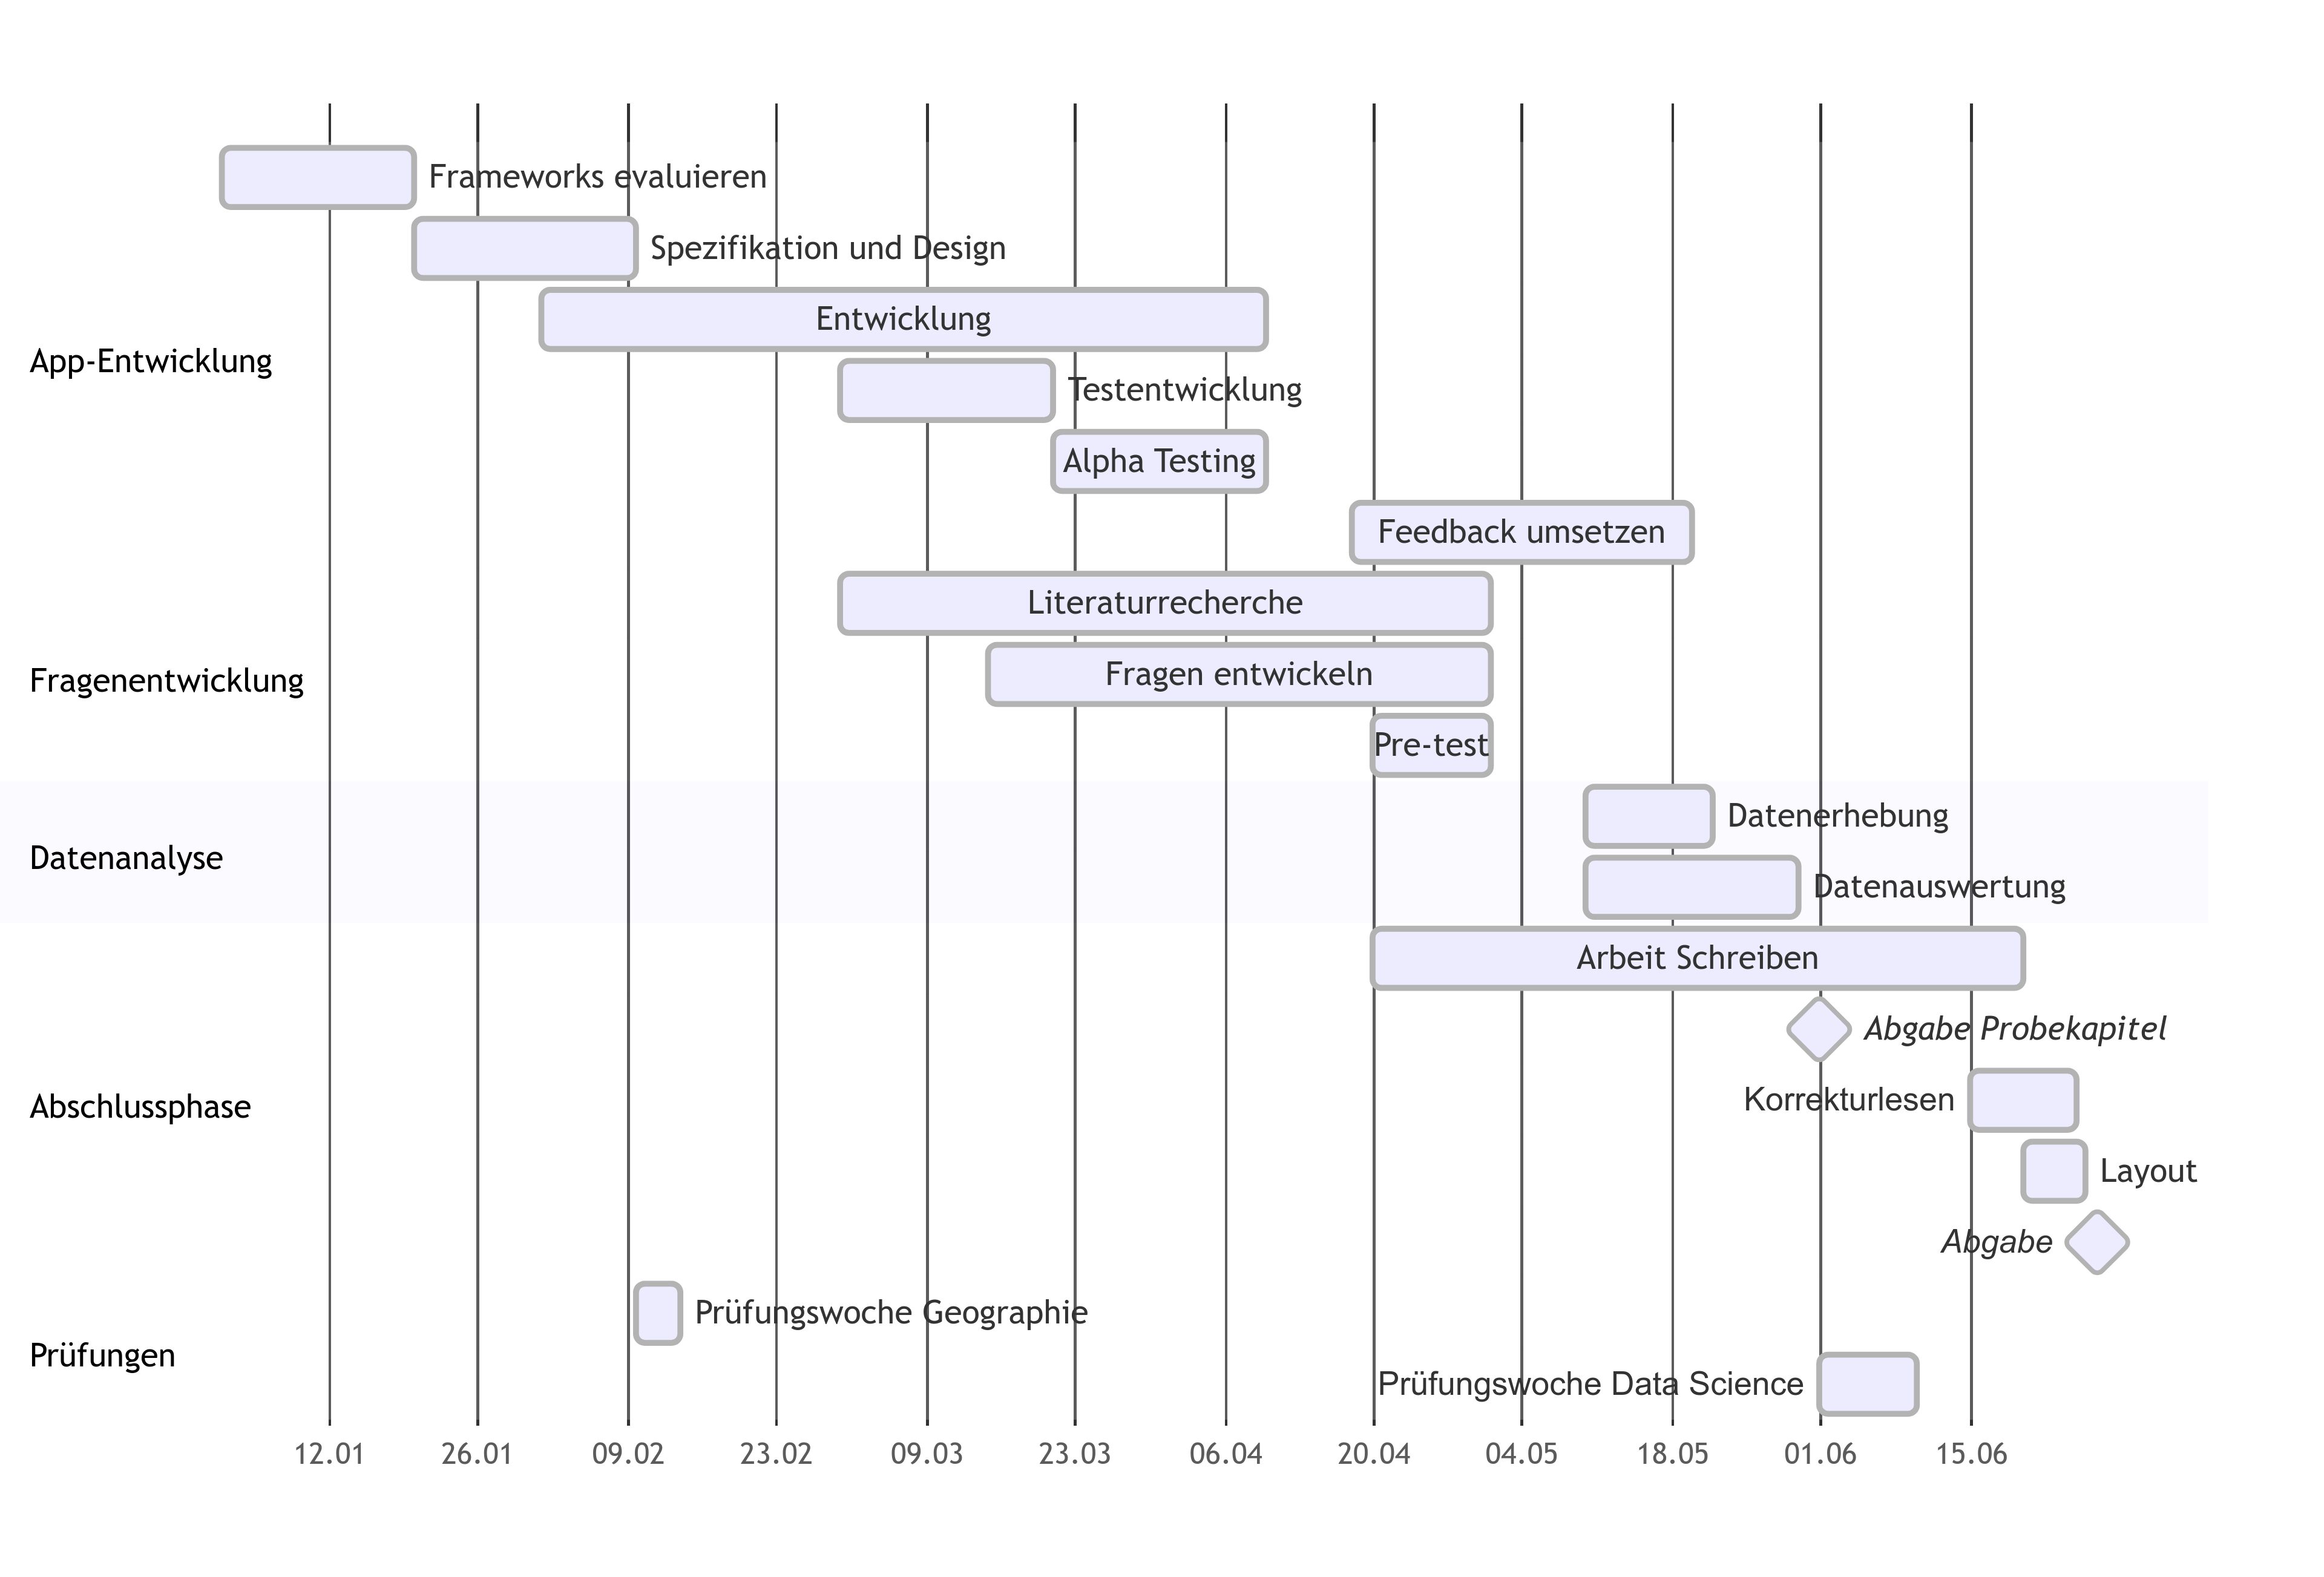
\includegraphics[width=1\linewidth]{Proposal/Timeline_BA_Lukas_Batschelet-2025-01-20-102140.png}
    \label{fig:timeline}
\end{figure}


\section{Risiken und Herausforderungen}

Die technische Implementierung der App stellt die grösste Herausforderung dar. Einige der geplanten Frameworks und Programmiersprachen sind mir nur begrenzt vertraut. Sollte sich im Verlauf des Projekts zeigen, dass eine vollständige Umsetzung im vorgesehenen Zeitrahmen nicht realisierbar ist, würde ich den Fokus nochmals verstärkt auf die Erarbeitung des Fragenkatalogs legen und eine einfachere, zu definierende Erhebung durchführen. Dies würde dann ermöglichen, eine ausführlichere Analyse und Präsentation der Daten durchzuführen.

Die geplante Erhebung von Daten zum Wohlergehen von Proband*innen erfordert eine ausführliche Prüfung datenschutzrechtlicher Grundlagen. Vorkehrungen wie Pseudonymisierung, eingeschränkte Standortgenauigkeit und die Möglichkeit zur Datenlöschung sind vorgesehen, um den gesetzlichen Vorgaben zu entsprechen.

\section{Kosten}
Für die Veröffentlichung der App in den offiziellen Stores fallen Gebühren für Entwicklerkonten an. Die Kosten betragen 99 USD pro Jahr für das Apple Developer Programm und eine einmalige 25 USD Gebühr für das Google Play Developer-Konto. Sonst ist mit keinen grösseren Ausgaben zu rechnen.


\section{Erwarteter Beitrag der Arbeit}
Diese Bachelorarbeit verbindet geographische Forschung mit technischen Entwicklungen und leistet einen Beitrag zur Methodik der intersektionalen Stadtforschung. Die erstellte App kann als Open-Source-Tool weiterentwickelt und für zukünftige Forschungsprojekte genutzt werden.

% ----------------- Bibliographie ------------------
\newpage
\PrintBib

\section*{Hinweis für den Einsatz von künstlicher Intelligenz (KI)}

Dieses Dokument wurde mithilfe von KI-basierten Tools überarbeitet. LanguageTool, ein KI-gestütztes Grammatik- und Stilprüfungswerkzeug, wurde verwendet, um Formulierungen zu verbessern und die Grammatik zu korrigieren. Chat-GPT von Open-AI wurde verwendet, um Feedback zur Klarheit und Strukturierung des Textes zu erhalten. Es wurde keine KI zur Erstellung von Originalinhalten verwendet.



\end{document}
